\documentclass[a4paper]{ltxdoc}
\usepackage[UTF8, heading=true, scheme=plain, linespread=1.2, zihao=-4, fontset=fandol]{ctex}

% counterwith重定义问题
\let\counterwithout\relax
\let\counterwithin\relax

\usepackage{float}
\usepackage[hidelinks]{hyperref}
\usepackage{geometry, parskip, seqsplit, fancyhdr, etoolbox, tocloft}
\usepackage{flafter, chngcntr, caption, multirow, graphicx}
\usepackage{minted} % 代码高亮模块,若不需要就删去
\usepackage[bottom]{footmisc} % 脚注放到页面最底部

\counterwithin{figure}{section} % 图的编号按section编排
\counterwithin{table}{section} % 表的编号按section编排
\DeclareCaptionFormat{smallformat}{\songti \small #1#2#3} % 宋体,五号

% 模板设置

\newcommand{\privacy}[1][密级]{#1} % 密级
\newcommand{\type}[1][【设计】]{#1} % 类型
\newcommand{\titleCn}[1][安徽省大学生学科竞赛在线报名系统设计与实现(微信小程序)]{#1} % 中文题目
\newcommand{\titleEn}[1][\LaTeX -based HFUT Thesis Template]{#1} % 英文题目

\newcommand{\keywordsCn}[1][小程序;管理系统;django;sqlserver;竞赛管理]{#1} % 中文关键字
\newcommand{\keywordsEn}[1][×××; ×××; ×××; ×××; ×××]{#1} % 英文关键字

\newcommand{\supervisor}[1][石雷]{#1} % 导师姓名
\newcommand{\studentID}[1][2015217003]{#1} % 学号
\newcommand{\studentNameCn}[1][李恒]{#1} % 填写中文姓名
\newcommand{\studentNameEn}[1][Hengliy]{#1} % 填写英文姓名

\newcommand{\finishedYear}[1][\the\year]{#1} % 论文完成日期: 年
\newcommand{\finishedMonth}[1][\the\month]{#1} % 论文完成日期: 月
\newcommand{\finishedDay}[1][\the\day]{#1} % 论文完成日期: 日


\newcommand{\department}[1][计算机与信息系]{#1} % 系名称
\newcommand{\major}[1][物联网工程专业]{#1} % 专业名称
\newcommand{\enrolmentYear}[1][2015级]{#1} % 入学年份



% 字号设置
\newcommand{\chuhao}{\fontsize{42pt}{\baselineskip}\selectfont}     % 字号设置
\newcommand{\xiaochuhao}{\fontsize{36pt}{\baselineskip}\selectfont} % 字号设置
\newcommand{\yichu}{\fontsize{32pt}{\baselineskip}\selectfont}      % 字号设置
\newcommand{\yihao}{\fontsize{28pt}{\baselineskip}\selectfont}      % 字号设置
\newcommand{\erhao}{\fontsize{21pt}{\baselineskip}\selectfont}      % 字号设置
\newcommand{\xiaoerhao}{\fontsize{18pt}{\baselineskip}\selectfont}  % 字号设置
\newcommand{\sanhao}{\fontsize{15.75pt}{\baselineskip}\selectfont}  % 字号设置
\newcommand{\sihao}{\fontsize{14pt}{\baselineskip}\selectfont}      % 字号设置
\newcommand{\xiaosihao}{\fontsize{12pt}{\baselineskip}\selectfont}  % 字号设置
\newcommand{\wuhao}{\fontsize{10.5pt}{\baselineskip}\selectfont}    % 字号设置
\newcommand{\xiaowuhao}{\fontsize{9pt}{\baselineskip}\selectfont}   % 字号设置
\newcommand{\liuhao}{\fontsize{7.875pt}{\baselineskip}\selectfont}  % 字号设置
\newcommand{\qihao}{\fontsize{5.25pt}{\baselineskip}\selectfont}    % 字号设置

% 下划线
\newcommand{\underlineFixlen}[2][3.5cm]{\underline{\makebox[#1][c]{#2}}}


% 中文摘要
\renewenvironment{abstract}{
\thispagestyle{empty} % 去掉页码
{
\begin{center}
\Large \songti \bfseries 摘\hspace{1em}要\vspace{1.1cm}
\end{center}
}
\setlength{\parindent}{2em}
\setlength{\parskip}{0em}
\setlength{\baselineskip}{22pt} % (宋体,小四;固定行距22磅,段前、段后均为0行间距。段落首行缩进2字符。)
\songti
}{
\setlength{\parindent}{0em}
\setlength{\parskip}{1em}
{\par \songti \bfseries{关键词:}}
\keywordsCn
\clearpage
}

% 英文摘要
\newenvironment{abstractEn}
{
\thispagestyle{empty} % 去掉页码
{
\begin{center}
\Large \bfseries ABSTRACT\vspace{1.5cm}
\end{center}
}
\setlength{\parindent}{1em}
\setlength{\parskip}{0em}
\setlength{\baselineskip}{22pt} % 22磅行距,首行缩进1字符,段前、段后均为0行间距
}{
\setlength{\parindent}{0em}
\setlength{\parskip}{1em}
{\par \bfseries{KEYWORDS:}}
\keywordsEn
\clearpage
}

% 目录名
\renewcommand\contentsname{
\begin{center}
\songti \Large \bfseries 目\hspace{1em}录 % (宋体,小二号,加粗;居中,单倍行距,段前0.5行、段后1.5行间距)
\end{center}
\vspace{1em}
}
% 插图清单
\renewcommand\listfigurename{
\begin{center}
\songti \Large \bfseries 插图清单 % (宋体,小二号,加粗;居中,单倍行距,段前0.5行、段后1.5行间距)
\end{center}
\vspace{1em}
}

% 表格清单
\renewcommand\listtablename{
\begin{center}
\songti \Large \bfseries 表格清单 % (宋体,小二号,加粗;居中,单倍行距,段前0.5行、段后1.5行间距)
\end{center}
\vspace{1em}
}

\renewcommand\refname{\heiti \sanhao \bfseries 参考文献}


% 目录引线设置
\renewcommand{\cftdotsep}{1.5} % 线的密度
\renewcommand{\cftsecdotsep}{1.5} % section引线
\renewcommand{\cftsecleader}{\cftdotfill{\cftsecdotsep}}
\renewcommand{\cftsecpagefont}{}

% 插图清单
\renewcommand{\cftfigpresnum}{\figurename\enspace}

% 表格清单
\renewcommand{\cfttabpresnum}{\tablename\enspace}

% 致谢
\newenvironment{acknowledge}{
\clearpage
\vspace*{-2em}
\phantomsection % 使得hyperref目录能够跳转到正确的位置
\addcontentsline{toc}{section}{致谢} % 添加到目录中
\begin{center}
 \songti \Large \bfseries 致谢\end{center}\vspace{1.1cm}
\setlength{\parindent}{2em}
\setlength{\parskip}{0.5em}
\setlength{\baselineskip}{22pt} % 22磅行距,首行缩进1字符,段前、段后均为0行间距
\songti
\par
}{
	\par
	\hfill 作者:\studentNameCn

	\hfill \finishedYear\enspace 年\finishedMonth\enspace 月\finishedDay\enspace 日
}

% 附录
\renewenvironment{appendix}{
\clearpage
\vspace*{-2em}
\phantomsection % 使得hyperref目录能够跳转到正确的位置
\addcontentsline{toc}{section}{附录} % 添加到目录中
\begin{center}
 \songti \Large \bfseries 附录\end{center}\vspace{1.1cm}
\setlength{\parindent}{2em}
\setlength{\parskip}{0.5em}
\setlength{\baselineskip}{22pt} % 22磅行距,首行缩进1字符,段前、段后均为0行间距
\songti
\par
}{
}

% 图名称
\renewcommand{\figurename}{图}
\renewcommand{\tablename}{表}


\captionsetup{
	labelsep=quad, % caption去掉分隔符:
	textformat=simple,
	format=smallformat,
}

\ctexset{
	space=auto,
	section = {
		format = \centering \heiti \sanhao \bfseries,
		aftername = \hspace{0.5em},
		afterindent = true,
	},
	subsection = {
		format = \heiti \bfseries,
		aftername = \hspace{0.4em},
		afterindent = true,
	},
	subsubsection = {
		format = \songti \bfseries,
		aftername = \hspace{0.4em},
		afterindent = true,
	},
}

\geometry{left=3cm, right=3cm, top=2.54cm, bottom=2.54cm}

\setmainfont{Times New Roman} % 英文字体


\begin{document}
	\begin{titlepage}
{\heiti 学\hspace{1.5em}号:\underlineFixlen[3.5cm]{\studentID} \hfill
	{\heiti 密\hspace{1.5em}级:\underlineFixlen[3.5cm]{\privacy}}}

\centering
{\vspace{1.7cm} 
\includegraphics{images/hfut_name.png}\vspace{0.3cm}}

{\LARGE \bfseries Hefei University of Technology}\vspace{1cm}

{\chuhao \heiti 本科毕业设计(论文)}\vspace{0.7cm}

{\LARGE \bfseries UNDERGRADUATE THESIS}\vspace{0.9cm}

{
\includegraphics[width=3.76cm, height=3.76cm]{images/hfut_logo.jpg}\vspace{1.3cm}}

{
\linespread{1.6}
\songti \sanhao
	{\bfseries 类\hspace{2em}型:}\underlineFixlen[8.8cm]{\type}\\
	{\bfseries 题\hspace{2em}目:}\underlineFixlen[8.8cm]{\titleCn}\\
	{\bfseries 专业名称:}\underlineFixlen[8.8cm]{\major}\\
	{\bfseries 入校年份:}\underlineFixlen[8.8cm]{\enrolmentYear}\\
	{\bfseries 学生姓名:}\underlineFixlen[8.8cm]{\studentNameCn}\\
	{\bfseries 指导教师:}\underlineFixlen[8.8cm]{\supervisor}\\
	{\bfseries 系名称\hspace{1em}:}\underlineFixlen[8.8cm]{\department}\\
	{\bfseries 完成时间:}\underlineFixlen[8.8cm]{\finishedYear 年\finishedMonth 月}\\
}


\end{titlepage}

	\begin{titlepage}
\centering

{
\parskip=0.5em
\linespread{1.25}
\LARGE \heiti
合\hspace{1.5em}肥\hspace{1.5em}工\hspace{1.5em}业\hspace{1.5em}大\hspace{1.5em}学\vspace{2.95cm}

\bfseries{本科毕业设计(论文)}\vspace{2cm}

\songti \bfseries{\titleCn} \vspace{6cm}
}

{
\parskip=0.5em \linespread{1.5}
\songti \sanhao
学生姓名:\underlineFixlen[8.8cm]{\studentNameCn}

学生学号:\underlineFixlen[8.8cm]{\studentID}

指导教师:\underlineFixlen[8.8cm]{\supervisor}

专业名称:\underlineFixlen[8.8cm]{\major}

系名称\hspace{1em}:\underlineFixlen[8.8cm]{\department}

\vspace{3.2cm}
\large
\finishedYear 年\finishedMonth 月
}


\end{titlepage}

	\begin{titlepage}
\centering
{
\parskip=0pt \linespread{1.25}
\sanhao \bfseries{A Dissertation Submitted for the Degree of Bachelor}\vspace{4.7cm}

\Large \bfseries{\titleEn} \vspace{1.8cm}}

{\sanhao By

\studentNameEn
\vfill
Hefei University of Technology

Hefei, Anhui, P.R.China

\finishedMonth\enspace Month, \finishedYear\enspace Year
\vspace{3cm}
}

\end{titlepage}

	\begin{titlepage}
\setlength{\parindent}{2em}
\setlength{\parskip}{0.5em}

{
\begin{center}
\heiti \Large
	\bfseries{毕业设计(论文)独创性声明}\vspace{1.2cm}
\end{center}
}

{
本人郑重声明:所呈交的毕业设计(论文)是本人在指导教师指导下进行独立研究工作所取得的成果。据我所知,除了文中特别加以标注和致谢的内容外,设计(论文)中不包含其他人已经发表或撰写过的研究成果,也不包含为获得\underlineFixlen[3cm]{合肥工业大学}或其他教育机构的学位或证书而使用过的材料。对本文成果做出贡献的个人和集体,本人已在设计(论文)中作了明确的说明,并表示谢意。

毕业设计(论文)中表达的观点纯属作者本人观点,与合肥工业大学无关。\vspace{1cm}

毕业设计(论文)作者签名:\hfill 签名日期:\hspace{2em}年\hspace{2em}月\hspace{2em}日
}

{
\vspace{3cm}
\begin{center}
\heiti \Large
	\bfseries{毕业设计(论文)版权使用授权书}\vspace{1.2cm}
\end{center}
}

{
本学位论文作者完全了解\underlineFixlen[3cm]{合肥工业大学}有关保留、使用毕业设计(论文)的规定,即:除保密期内的涉密设计(论文)外,学校有权保存并向国家有关部门或机构送交设计(论文)的复印件和电子光盘,允许设计(论文)被查阅或借阅。本人授权\underlineFixlen[3cm]{合肥工业大学}可以将本毕业设计(论文)的全部或部分内容编入有关数据库,允许采用影印、缩印或扫描等复制手段保存、汇编毕业设计(论文)。

(保密的毕业设计(论文)在解密后适用本授权书) \vspace{1.5cm}

学位论文作者签名:\hfill 指导教师签名:\hspace{7em}

签名日期:\hspace{2em}年\hspace{2em}月\hspace{2em}日\hfill 签名日期:\hspace{2em}年\hspace{2em}月\hspace{2em}日
}


\end{titlepage}

	
	\begin{abstract}
		随着互联网的飞速发展,各行各业都在深入的融合互联网。而随着智能手机的普及,移动互联网的概念又进入我们的生活,移动互联网极大的方便了我们的工作与生活。
		
		2019年最新统计显示,微信用户已经达到10亿人次,而微信小程序用户也已经达到6亿。微信小程序具有轻量级的特点,使得更多的用户愿意去使用,简单容易上手,操作流程简单。具有轻便快捷、随到随用、用完即走的特性,符合我们轻便快捷的生活节奏,是新时代移动服务提供的新形式。
		
		研究会承办安徽省高校7类计算机竞赛。每项赛事每年都会举办一次,省内高校都可以注册登录报名。
		竞赛报名系统承担开发于2016年,目前已经不能完全适应七大赛事每年不断增加的报名需求和压力,因此迫切需要在原有基础上开发新的系统。为了增加报名系统的轻便快捷的特点,开发出报名系统的微信小程序端。
		
		本系统使用小程序技术+Django+sqlserver架构和restfulAPI接口标准。可以实现多角色注册,竞赛报名,参赛队伍管理,在线审核,在线查分,添加竞赛,竞赛流程管理等功能。本文主要阐述了报名小程序系统的设计与实现。
	\end{abstract}
	
	\begin{abstractEn}
			\seqsplit{
			With the rapid development of the Internet, all walks of life in the in-depth integration of the Internet.With the popularity of smart phones, the concept of mobile Internet has entered our life. Mobile Internet has greatly facilitated our work and life.}
		
			\seqsplit{
			According to the latest statistics in 2019, WeChat users have reached 1 billion, while WeChat small program users have also reached 600 million.WeChat small program has the characteristics of lightweight, so that more users are willing to use, simple and easy to use, simple operation process.It is light and fast, ready to use and ready to go. It is in line with our light and fast pace of life and a new form of mobile service in the new era.}
			
			\seqsplit{
			The association will undertake 7 kinds of computer competitions of colleges and universities in anhui province.Each event is held once a year, and colleges and universities in the province can register for it.}
			
			\seqsplit{
			The competition registration system was developed in 2016. At present, it is unable to fully adapt to the increasing registration demands and pressures of the seven major competitions every year. Therefore, it is urgent to develop a new system based on the original one.In order to increase the sign up system's portable and quick characteristic, the development sign up system's WeChat small program end.}
			
			\seqsplit{
			This system USES small program technology +Django+sqlserver architecture and restfulAPI interface standards.Multi-role registration, competition registration, team management, online audit, online scoring, add competition, competition process management and other functions.This article mainly elaborated the registration small procedure system design and the realization.}

	\end{abstractEn}
	
	% 目录
	{
		\tocloftpagestyle{empty}
		\setlength{\cftfignumwidth}{3.5em}
		\setlength{\cfttabnumwidth}{3.5em}
		\clearpage
		\tableofcontents
		\addtocontents{toc}{\protect\thispagestyle{empty}}
		\pagenumbering{gobble}
		
		\clearpage
		\listoffigures
		
		\clearpage
		\listoftables
		
		\pagenumbering{arabic}
	}
	
	% 设置页眉
	\newgeometry{left=2.8cm, right=2.8cm, top=3cm, bottom=3cm}
	\fancyhead{}
	\chead{\small 合肥工业大学毕业设计(论文)\vspace{0.3cm}}
	\pagestyle{fancy}
	
	% 正文
	{
		\setcounter{page}{1}
		% 重写section指令以便设置section段前1行间距,分页
		\pretocmd{\section}{\clearpage \vspace*{-2.0em}}{}{}
		
		\setlength{\parindent}{2em}
		\setlength{\parskip}{0.5em}
		\setlength{\baselineskip}{22pt}
		
		\section{绪论}
		\subsection{项目背景}
		现在,随着移动互联网信息技术的发展以及“互联网+”的深入发展,移动互联网已经深入我们每个人的工作与生活,2019年5G网络的建设已经提上了日程规划,国内三大运营商已经开始了5G 网络的布局。移动互联网时代已经到来。网络技术的发展以及。加强移动互联网终端应用的创新和建设,有利于各事业单位、企业为用户提供更好的服务。手机作为移动移动互联网的主要动力,为我们提供了无数的便捷服务,而微信作为使用度最高的社交工具 ,在移动应用领域拥有庞大的用户基础,截至2019年3月,微信用户已经超过10亿,目前移动开发主要为ios,Andriod App和微信小程序,而微信小程序相比前者具有更好的的灵活性,提供一种新的链接用户与服务方式,用户只需要扫一扫或搜一下即可打开应用;使用完毕无需关闭卸载,简化了操作步骤,节省时间,提高了用户体验,并且微信小程序可以在各种平台上使用,开发更加简单。移动服务已经成为当今服务提供的主流。
		
		\subsection{项目意义}
		安徽省高等学校计算机教育研究会是在安徽省教育厅领导、安徽省民政厅领导的指导,督促,鼓励和关注下,在全国高等学校计算机基础教育研究会及谭浩强教授的关心下,在华东高校计算机基础教育研究会及张森教授的督促和直接帮助下,在中国铁道出版社、清华大学出版社等出版单位的大力支持下筹备组建成立的。 安徽省高等学校计算机教育研究会的主管单位是安徽省教育厅,挂靠单位是安徽省合肥工业大学。目前,研究会承办安徽省高校计算机类竞赛有七个,分别是程序设计竞赛,单片机竞赛,机器人竞赛,信息安全作品赛、网络攻防赛、大数据与人工智能应用赛以及数字媒体创新设计赛。每项赛事每年都会举办一次,省内高校都可以注册登录报名。研究会现有网站和报名系统(网址:http://www.ahjsjjy.com)开发于2016年,目前已经不能完全适应七大赛事每年不断增加的报名需求和压力,并且现有系统学生报名与老师管理以及管理员的审核都只能在电脑网页端完成因此迫切需要在原有基础上开发新的系统,并为了提供移动式便捷办公的需求,开发此微信小程序。可以让用户能够在移动端完成竞赛的报名及管理,提高了工作的效率,更加人性化。使得安徽省学科竞赛的开展更快捷高效。
		
		\subsection{项目简介}
		功能方面,为了解决上述需求,本项目设计并开发了安徽省学科竞赛报名管理微信小程序。功能方面本系统可以分成学生、老师、管理员三个角色模块,学生模块由学生注册登陆,学生可以修改个人信息、密码,浏览安徽省内的比赛项目,加入比赛队伍以及提交竞赛作品,老师模块由老师注册登陆,老师可以修改个人信息、密码,可以创建竞赛队伍并根据队员姓名添加队员,还能够修改队伍信息以及报名比赛。管理员模块可以管理审核注册及修改待审核信息的用户、创建及修改待审核信息的竞赛队伍,还可以创建新的竞赛、修改竞赛信息以及控制报名系统开放时间段。
		
		技术方面,本项目采用B/S(client/server)架构,客户端使用微信小程序技术,服务器端采用Django框架、sqlserver数据库,客户端与服务器端通信接口参照了restFul设计标准,充分利用Django提供的MTV模型与ORM数据库操作,缩短了开发时间,降低了代码复杂度,增加了系统的稳定性与可维护性。
		
		\subsection{论文主要结构}
		本论文主要介绍了安徽省大学生学科竞赛小程序的主要功能、系统设计、系统展示和使用介绍。本文按照需求分析,可行性分析,初步设计,详细设计,形成文档,建立初步模型,编写详细代码以及测试修改的基本软件开发步骤,结合具体的已实现的软件,进行了分析介绍。
		
		本文总共分为6章,篇章结构为:
		
		第一章为引言,主要从客观的角度阐述了项目课题的来源以及研究背景。
		
		第二章为功能需求和总体设计,主要介绍了该课题的需要实现的功能需求,即协议相关内容,以及项目的整体设计思路。
		
		第三章为系统技术以及框架介绍,主要介绍了在系统中所用到的主要技术手段以及实现功能的辅助框架情况。
		
		第四章为详细结构设计,主要以项目中各系统下的各模块为单一对象,对该对象做一些技术实现和逻辑介绍。
		
		第五章为系统测试分析,主要介绍测试项目的功能逻辑以及并发能力的过程和结果。
		
		第六章为结论和展望,主要总结了该项目的完成情况以及未来的发展情况。
		
		
		\section{相关技术以及框架介绍}
		\subsection{微信小程序技术}
		微信小程序简称小程序,英文名WeChatMiniProgram(XCX),由腾讯微信事业部进行开发。微信小程序最大的特点是不需要用户去应用商店进行下载安装,可以直接在聊天分享内容中点击进入,或者扫描二维码,响应速度快,几乎不需要等待时间就可以使用全部功能,并且退出后不占用手机内存。微信小程序有三个特点:1.不需要下载安装即可使用;2.用户“用完即走”,不用关心是否安装太多应用;3.用将无处不在、随时可用。	
		
		微信小程序的发展速度极快,从2016年1月微信总裁张小龙向外界透露微信将要研发出不同于APP的微信应用号,此为微信小程序的前身,到2017年月,腾讯公司财务报告中指出微信的月活跃用户已达到 9.8 亿,已经是当前移动端社交软件中最高活跃用户数的第一名,越来越多的企业主开始注册微信小程序,注册量达2000多万,这些可观的数据为微信“小程序”的发展奠定了扎实的平台基础。
		
		基于上述描述,微信小程序作为研究会报名系统的客户端需求实现的工具再合适不过了,用户在注册报名和查看信息时,打开小程序扫一扫用完即关,不需安装另外的 APP,也不需要打理,报名完成就结束使用。
		
		\subsection{python 与 Django开发框架}
		python是一种面向对象、解释型计算机程序设计语言,语言可读性强、代码可移植性高,并有强大丰富的代码库支持,使得开发迅速。Django是Python的代表性全能框架,Django的设计目标是快速开发web应用,它提供了较多内置的模块,cache缓存模块、以及自主管理后台admin模块、自定义views模块、URL路由配置模块、数据库orm模块。Django拥有一套完整的官方文档,还拥有多个活跃的社区,提供了全套的解决方案,Django工作机制是用户通过浏览器访问请求一个页面,中间件对request做一些处理或者直接发起response,路由配置模块通过urls.py将请求的url链接与对应的views模块匹配起来,views模块中通过自定义的方法操作settings模块中配置的数据库,将数据库查询出的内容结合static静态文件和Template中页面文件一起返回,通过浏览器渲染显示给用户。
		
		\subsubsection{Django MTV模型}
		Django是一个基于MVC构造的框架。但是在Django中,控制器接受用户输入的部分由框架自行处理,所以Django里更关注的是模型(Model)、模板(Template)和视图(Views),称为 MTV模式。架构的主要框图如下:
		
		% \begin{table}[!htb]
		% \centering
		% \caption{MTV层次功能表}
		% \begin{tabular}{ccccc}
		% \hline
		% 年度                    					   & 职责  \\ \hline
		% \multirow{2}{*}{模型(Model)} 			   &处理与数据相关的所有事务:如何存取、如何验\\
		% 										   &证有效性、包含哪些行为以及数据之间的关系等。  \\\hline
		% \multirow{2}{*}{模板(Template)}   		   &处理与表现相关的决定:如何在页面\\
		% 										   &或其他类型文档中进行显示。  \\ \hline
		% \multirow{2}{*}{视图(View)}  			   &存取模型及调取恰当模板的相关逻辑。\\
		% 										   &模型与模板的桥梁。\\ \hline
		% \end{tabular}
		% \end{table}
		
		\begin{figure}[!htb]
			\centering
			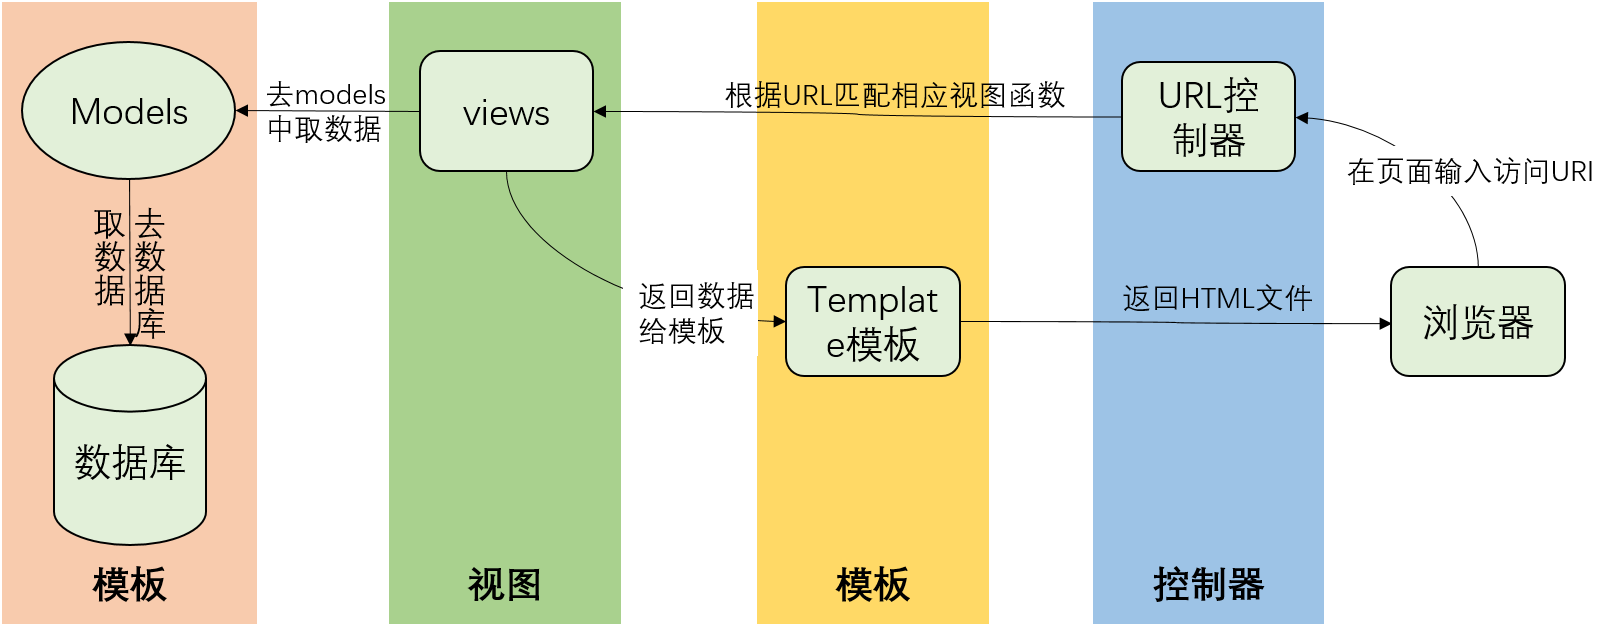
\includegraphics[width=1.0\linewidth]{images/5.png}
			\caption{Django架构图}
		\end{figure}
		
		从以上表述可以看出Django视图不处理用户输入,而仅仅决定要展现哪些数据给用户,而Django模板仅仅决定如何展现Django视图指定的数据。或者说,Django将MVC中的视图进一步分解为 Django视图和Django模板两个部分,分别决定“展现哪些数据”和“如何展现”,使得Django的模板可以根据需要随时替换,而不仅仅限制于内置的模板。
		
		\subsubsection{Django URL路由分配系统}
		
		Django框架除了上述的MTV模型还有一个urls分发器,它的作用是将一个个URL的页面请求分发给不同的view处理,view再调用相应的Model和Template。
		
		Django路由分发的工作流程:
		
		1、客户端发送请求(get/post/put/delete)经过web服务器、Django中间件、 到达路由分配系统 
		
		2、路由分配系统根据提取 request中携带的的url路径(path)与视图函数映射关系列表中,匹配到1个视图函数,foo(request)执行;
		
		3、视图函数 使用原生SQL或者ORM去数据库拿到数据,在服务端进行渲染(模板+数据渲染)
		
		4、视图函数return一个 response对象 返回客户端
		
		\subsubsection{Django ORM数据库操作}
		Django的一个强大的功能是它的对象关系映射Object-Relational Mapping(ORM),它允许用户就像使用 SQL一样去和用户的数据库交互。Django采用了基于ORM操作数据库的方法,Django使用ORM操作数据库的相关配置、增删改查等相关操作技巧。只需要面向对象编程,不需要面向数据库编写代码。对数据库的操作都转化成对类属性和方法的操作。不用编写各种数据库的sql语句。实现了数据模型与数据库的解耦,屏蔽了不同数据库操作上的差异.不在关注用的是哪种数据库等,通过简单的配置就可以轻松更换数据库,而不需要修改代码。
		
		\begin{figure}[!htb]
			\centering
			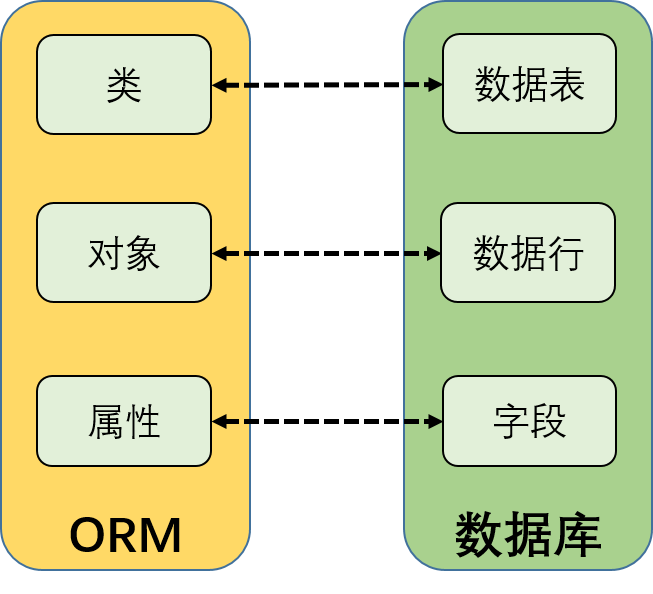
\includegraphics[width=0.5\linewidth]{images/6.png}
			\caption{ORM-数据库映射图}
		\end{figure}
		
		
		\subsection{restfulAPI标准}
		REST是“REpresentational State Transfer”的缩写,中文翻译成“表现状态转换”【1】。该规范并不是一种新技术的或者新组件或者新服务的创造,而是一种理念的创新,将现有的WEB技术特征和能力进行整合,使其符合一些准则和约束。如果一个架构符合REST规范,就称它为RESTful架构【3】。
		
		与面向对象的编程语言中一切都是对象一样,在REST规范的世界里,一切都是资源;而与编程语言中的对象不一样的是,在REST规范中,资源只定义了有限的方法。理解REST规范的重点在于理解什么是资源。可以把资源理解成一种对象,包括对象的类型、数据、关系、操作等等。资源要能够被识别,就需要给每个资源分配一个唯一的标识。在REST规范中,这个唯一的标识是URI(Uniform Resource Identifier)【1】。URI的最大特点是可读性强,能够降低前后端开发人员的沟通次数,提高效率。
		
		REST规范规定要使用统一的接口原则,也就是上文提到的资源只限定了有限的方法,无论什么资源,都可以通过使用限定的这几类方法进行资源的访问。REST中规定了六种类型的请求方式:GET、POST、PUT、DELETE、HEAD、OPTIONS,正好与CRUD(Create-Retrieve-Update-Delete,增删改查)四种操作相对应,例如,GET(查)、POST(增)、PUT(改)、DELETE(删)。例如:http://www.xxx.abc/em⁃ployees/c001表示的是编号为001的员工。
		
		
		%例如:
		
		%\begin{center}
		%\begin{table}[!htb]
		%\centering
		%\caption{Restful简表}
		%\begin{tabular}{ccccc}
		%\hline
		%REST请求                    				& 描述\\ \hline
		%\multirow{1}{*}{GET:/employees} 		&获取所有员工的信息\\ \hline
		%\multirow{1}{*}{GET:/employees/001}     &获取ID为001的员工信息\\ \hline
		%\multirow{1}{*}{PUT:/employees/001}     &更新ID为001的员工信息\\ \hline
		%\multirow{1}{*}{DELETE:/employees/001}  &删除ID为001的员工信息\\ \hline
		%\multirow{1}{*}{POST:/employees/001}    &创建ID为001的员工信息\\ \hline
		%\end{tabular}
		%\end{table}
		%\end{center}
		
		%本系统使用的RestFul标准
		
		% 代码示例\footnote{本系统restful}
		% \begin{minted}[
		% 	frame=lines,
		% 	framesep=2mm,
		% 	baselinestretch=1.2,
		% 	fontsize=\footnotesize,
		% 	linenos
		% ]{python}
		
		% HTTP/1.1 200 OK
		% Content-Type: application/json
		% Content-Length: 234
		
		% {
		% 	"url":"/api/categoreis/1"
		% 	"label":"duty"
		% 	"functions":[
		% 		{
		% 			"label":"",
		% 			"function_key":"800",
		% 			"url":"api/function/800"
		% 		}
		% 	]
		% }
		% \end{minted}
		
		\subsection{sqlserver}
		SQL Sever2012 是一个安全可靠的、功能全面、数据集成的数据平台,能支持企业级组织机构提供商业智能的解决方案,管理海量企业数据。SQL Server2012功能强大,工具丰富,页面设计美观方便使用,并且可扩展性好,在移动设备上同样能实现数据库的调用和数据的更新等,支持多平台管理,同时可以降低程序逻辑结构的复杂性,使开发变得简单便捷。SQL Server 作为关系型数据库管理系统,有着强大的实用功能。安全性是信息系统开发需要考虑的重要需求,SQL  Server 数据库的安全性能很高,可以防止其他用户因对数据库的不当使用所造成的数据泄露、数据非法修改、数据破坏等。数据库的安全与否直接关系到计算机系统包括网络系统、操作系统的安全与否,它们之间是相互支持、紧密联系的。SQL Server数据库具有多个方面、多个层面的安全策略。在数据管理方面SQL Server在数据备份、数据恢复、容灾等多个方面。此外它还提供用户身份验证、权限管理等用户管理层面的安全策略。 
		
		本章先对微信端的微信交互接口进行分析设计,再从学生,老师,管理员三个角色角度进行需求分析,其中与微信交互接口的设计是其他功能模块的前置条件,所有功能模块最终都是通过微信交互接口与用户产生直接交互。在需求分析明确后在前两章的研宄基础上,对基于Django的web系统框架,进行了分层系统设计,使其具有通用性。
		
		\section{需求分析与总体设计}
		
		\subsection{需求分析}
		需求分析是软件设计阶段的一项重要活动,也是软件生命周期中的一个非常重要环节,其目标是把用户对于开发软件所提出的“要求”或“需要”进行分析与整理,确定软件需要实现什么样的功能,完成哪些工作。
		
		\subsubsection{软件需求分析}
		安徽省大学生学科竞赛微信端报名系统的需求来源于现有网站的诸多缺点与竞赛管理移动办公的需求。将原本只能在电脑端操作的报名及管理工作放在手机上,这可以极大的简化办公的流程。针对临时的报名审核管理员不需要打开电脑登陆网站,在手机上就可以晚上大部分工作。根据以上分析与如今企业开发中使用的主流框架,本系统采用了B/S架构。考虑到系统的业务连续性客户端采用了小程序最新的开发文档。
		
		在服务器端,本系统采用的Django提供后端服务,而Django采用python语言进行开发,所以需要在服务器端安装python解释器。同时由于需要服务器对外提供web服务,需要安装服务器软件提供web服务,本文选择较为流行的可选服务器软件为Apache、Nginx等。数据库沿用教研会管理网站现有的sqlserver数据库服务器,与web端共享管理数据。通过Django处理客户端页面传入后台的数据,操作sqlserver完成数据的增删改查。
		
		在客户端,微信小程序不同于其他APP之处在于,其在微信中运行,通过微信调用本地设备接口或调用微信功能,而无需单独下载安装,只需在微信中检索后即可使用,因此在客户端仅需要安装微信并能够正常访问网络。
		
		\subsubsection{系统可行性分析}
		可行性分析的目的是花费最小的代价在尽可能短的时间确定系统能否解决问题,这是对系统简化和设计的过程,也是在较高层次上以较为抽象的方式进行系统分析和设计的过程。微信竞赛报名系统的开发,要考虑到操作的是否足够简单、技术是否可行、经济是否足够。
		(一)操作可行性:本系统的界面简介美观、用户不用经过培训就知道如何操作。
		
		(二)技术可行性:Django是目前火热的后端框架,许多著名的网站就是使用Django框架开发的。并且因为其强大的功能,能够简化代码开发阶段的问题,例如ORM操作可以简化数据库操作极其方便,并能够忽视掉后台数据库的类型,只用更新配置不用更新业务代码。
		
		(三)经济可行性:本系统开发完成,使用本地测试后,部署在研究会现有服务器器上,与现有web端后台同时运行提供服务。不需要额外费用。
		
		故本系统符合操作可行性、技术可行性、经济可行性。
		
		\subsubsection{功能需求分析}
		本项目的目的就是在为安徽省学科竞赛报名管理系统创建一种移动轻量式办公环境,设计并开发一个基于微信小程序的移动办公平台,为学生,老师和管理员三种角色开展竞赛活动提供服务,同样的微信报名系统,学生登陆可以浏览比赛,加入已经创建好的竞赛队伍,老师登陆可以创建队伍、管理竞赛队伍、报名比赛。管理员登陆可以创建金属盖、编辑竞赛信息、队伍审核、系统定时开放、会员管理。面对这些需求,我们从三种角色的角度进行分析,分别是学生,老师,管理员。

		
		\textbf{(一)管理员用户模块功能如下}
		
		创建竞赛:管理员需要在平台上创建竞赛,包括竞赛的名称、竞赛时间、子竞赛名称、竞赛分类等相关信息。创建竞赛是竞赛管理的首位,只有创建了竞赛,并且竞赛在报名期间,老师才登陆小程序,才可以给相关队伍报名竞赛。
		
		编辑竞赛信息:在创建竞赛后,管理员还有一种修改竞赛信息的需求,在竞赛的名称和竞赛的规则在进一步确定和完善后可能需要修改竞赛信息,可以随时修改竞赛介绍、竞赛规则、竞赛队伍数量、竞赛举行时间、报名时间段等信息。
		
		竞赛队伍审核:竞赛队伍在创建后不能立即报名,其信息需要符合要求,得到管理员的审核。
		
		系统定时开放:报名系统需要在指定时间段定时开放,在竞赛报名时间结束后,拒绝一切报名服务。
		
		会员管理:会员在注册后信息不能确定是否符合要求,需要得到管理员的审核。审核通过后才可以进行后续服务。
		
		\textbf{(二)老师用户模块功能如下}
		
		注册/登陆:注册/登陆,修改用户的基本信息。
		
		创建队伍:队伍的创建是各个学校的老师根据自己学校提交上来的名单自行创建的,老师需要在移动平台上创建自己学校的竞赛队伍。
		
		队伍管理:在竞赛队伍创建后,老师还需要管理自己带领的队伍,包括竞赛报名,队伍信息修改,在竞赛系统开通的时间段内进行竞赛队员的添加或删除等操作。
		
		报名比赛:竞赛队伍的创建可以随时创建,但是报名只能在意向竞赛开通报名时间段内进行报名。
		
		\textbf{(三)学生用户模块功能如下}
		
		注册/登陆:注册/登陆,修改用户的基本信息。
		
		浏览竞赛项目:学生用户在竞赛报名系统上,首要需求需求是对平台上的竞赛进行查看,选择自己感兴趣的竞赛,了解其详细信息与报名资料。因此报名系统首先要考虑如何呈现这些竞赛项目,以方便学生进行查看、阅读。
		
		提交作品:在队伍报名后,队伍中任意一个队员均可以提交作品,并填写作品介绍。作品大小与作品介绍字数均需要得到限制。
		
		\subsubsection{系统性能需求分析}
		微信学科竞赛报名系统针对报名功能的设计和编写代码、系统最终应该满足竞赛浏览、队伍组件、竞赛报名等所有的基本功能,因为要面向正式的工作环境,还要能够保证系统在长时间运行的情况下的稳定,以及频繁访问所产生的大量数据处理的准确性,保证系统的安全、保证用户能够在短时间能就能上手,操作简单。 
		
		\subsubsection{目标系统要求}
		目标系统应该达到以下要求: \\
		(一)时间经济性。优化逻辑设计与物理设计,使系统运行效率高、反应速度快微信课堂练习系统。\\
		(二)可靠性。能够连续准确的处理业务,有较强的容错性。\\
		(三)可理解性。用户能够容易理解和使用微信课堂练习系统。\\
		(四)可维护性和适应性。系统应该容易修改、容易扩充、容易维护,能够适应不断变化的业务需求。\\
		(五)可用性。系统功能齐全,能够完全满足业务需求。\\
		
		%%%%%%%%%%%%%%%%%%%%%%%%%%%%%%%%%%%%%%%%%%%%%%%%%%%%%%%%%%%%%%%%%%%%%%%%%%%%%%%%%%%%%%%%%%%%%%%%%%%%%%%%%
		\subsection{总体设计}
		系统的总体设计是对系统进行一个自上向下或自下向上的一个总体的概括与设计。将系统进行总体的架构之后,对系统的每一个层级进行细化,并介绍实现的方法。系统的总体框架相当于系统的骨骼,是系统支撑的部分。系统设计是后续详细设计的基础,通过系统设计可以方便后续代码的编写。 
		
		总体设计是一个设计者依据用户交流的流程,一个根据用户需求来构成交互框架和视觉框架的流程,其结果决定了交互控件的布局、界面元素的分组和界面整体样式的页面框架图。这是一个在用户和设计者之间搭起桥梁,使用户和设计者达成共识,将用户目标与需求转换成详细的界面设计解决方案的重要阶段。
		
		总体设计的主要目的是根基于需求分析阶段得到的信息转换为软件结构和数据结构。设计软件结构的具体任务是:将一个繁杂的系统按功能进行模块区分、建立各个模块之间的层级结构及调用关系、确定模块之间的接口等。
		
		本系统根据之前的需求分析、共分为三大模块,老师模块、学生模块、管理员模块。总体设计框架图3.1所示:
		
		\begin{figure}[!htb]
			\centering
			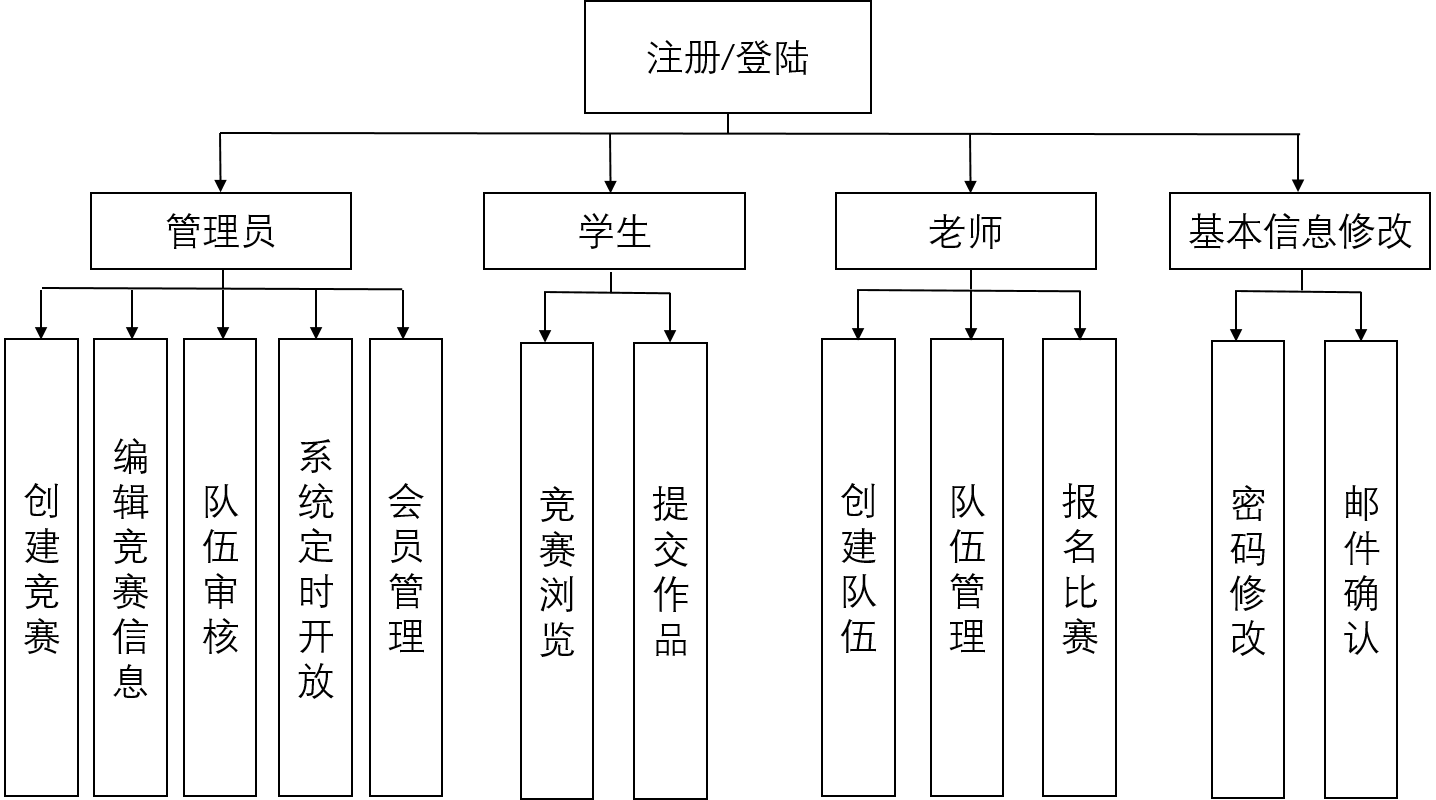
\includegraphics[width=0.95\linewidth]{images/1.png}
			\caption{需求分析框图}
		\end{figure}
	
		\subsubsection{注册/登陆模块设计}
		\begin{figure}[H]
			\centering
			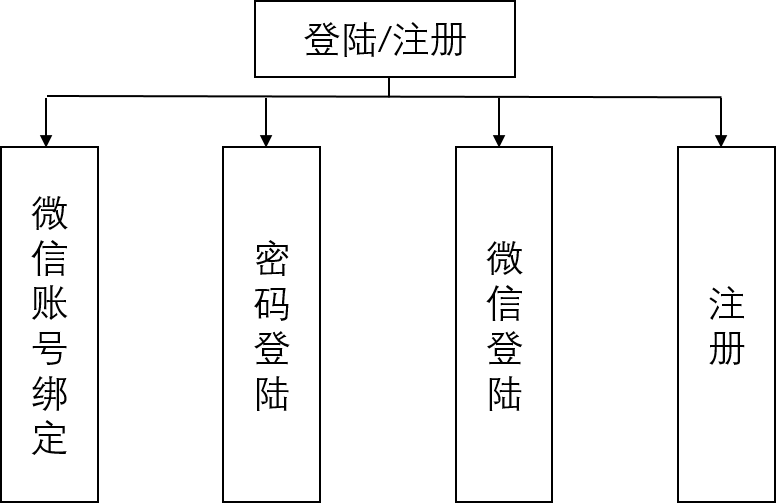
\includegraphics[width=0.7\linewidth]{images/1-4.png}
			\caption{注册/登陆模块功能图}
		\end{figure}
		
		用户打开小程序后,如果绑定过微信账号的用户将直接进入菜单界面,未绑定微信账号或未注册的用户将进入登陆界面,登陆时可选择账号密码登陆或者小程序登陆。当输入账号密码登陆时会提示是否绑定微信小程序。用户选择是则跳转进行绑定,如果选择否则直接进入菜单界面。
		
		如果未注册则在登陆界面点击注册进入注册界面,填入个人信息。并选择是否绑定微信账号。信息填写完成提交后需要等待管理员审核通过才能进行登陆操作。
	
		\subsubsection{学生模块设计}
		\begin{figure}[H]
			\centering
			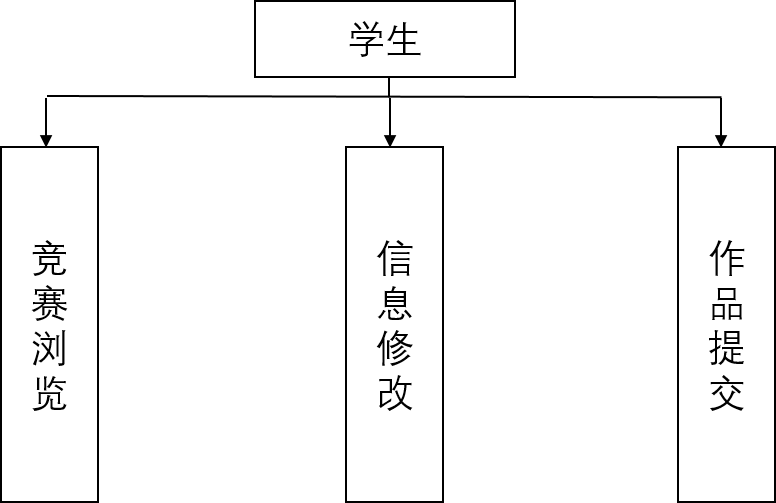
\includegraphics[width=0.7\linewidth]{images/1-2.png}
			\caption{学生模块功能图}
		\end{figure}
		学生模块包括学生在微信端的登陆、在微信端修改密码、修改个人信息、竞赛项目浏览、提交竞赛作品、成绩查询等功能。
		
		学生模块流程包括学生如果在微信端绑定账号,则可以不输入账号密码直接进入操作页面。点击修改密码会进入修改密码界面,在修改密码界面输入旧密码和新密码,然后点击修改密码,返回登陆页面并会发送警告邮件给绑定的邮箱。学生点击修改个人信息,进入个人信息页面,可以修改查看姓名、性别,查看账号和学校专业,但是编号和学校专业不能修改。
		
		点击竞赛浏览会进入到竞赛列表页面,里面包含了从后台传来的现有的竞赛简要信息列表,竞赛信息包括竞赛名称、竞赛报名时间、竞赛地点等简要信息,学生点击感兴趣竞赛进行详细了解。
		
		竞赛的详细信息菜单里面列出了竞赛的名称、简介、报名时间段、比赛时间、比赛联系方式、比赛QQ群等信息。
		
		点击提交作品会进入作品提交页面,此页面会显示已经提交的作品信息,如果在比赛时间段内仍可提交作品,则新提交的作品会覆盖已有的作品。
		
		\subsubsection{老师模块设计}
		\begin{figure}[H]
			\centering
			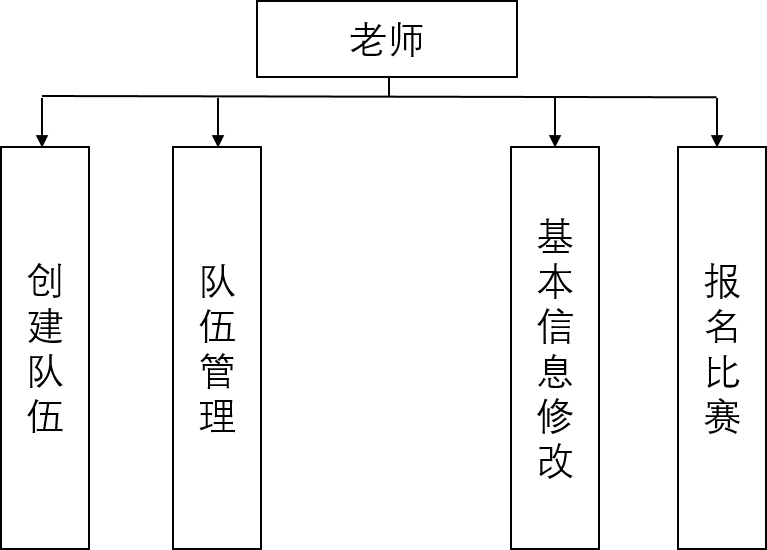
\includegraphics[width=0.7\linewidth]{images/1-3.png}
			\caption{老师模块功能图}
		\end{figure}
		老师模块包括老师在微信端的登陆、在微信端修改密码、修改个人信息、创建队伍、对已有竞赛队伍进行管理包括删除队伍,修改队伍信息,增加或删除队伍成员、报名比赛等功能。
		
		点击修改密码会进入修改密码界面,在修改密码界面输入旧密码和新密码,然后点击修改密码,返回登陆页面并会发送警告邮件给绑定的邮箱。老师点击修改个人信息,进入个人信息页面,可以修改查看姓名、性别,描述。
		
		老师模块流程包括教师在微信端如果绑定账号,则可以点击操作直接进入菜单页面、在菜单页面选择需要完成的操作。
		
		点击队伍管理会进入到队伍列表页面,里面包含了从后台传来的现有的队简要伍信息列表,队伍信息包括队伍名称、队伍成员数、队伍参加竞赛的名称、队伍是否已报名等简要信息。
		
		点击需要管理的队伍会进入队伍信息详情页,里面包含队伍的详细信息,包含了队伍的名称,队伍成员数、队伍参加比赛的名称、队伍是否已经报名、队伍成员数、队伍指导老师、队伍教练等详细信息。点击报名会弹出正在开放报名的比赛列表,老师选择学生意向报名竞赛并依次选择竞赛组别进行报名。点击添加队员,会弹出搜索框,在搜索框中输入学生姓名并搜索会列出所有同名的学生,老师比较学生信息后选择正确的学生进行添加。
		
		队伍详情信息中可以删除此队伍,点击后会弹出删除警告,确认删除后方可删除。
		
		\subsubsection{管理员模块设计}
		\begin{figure}[H]
			\centering
			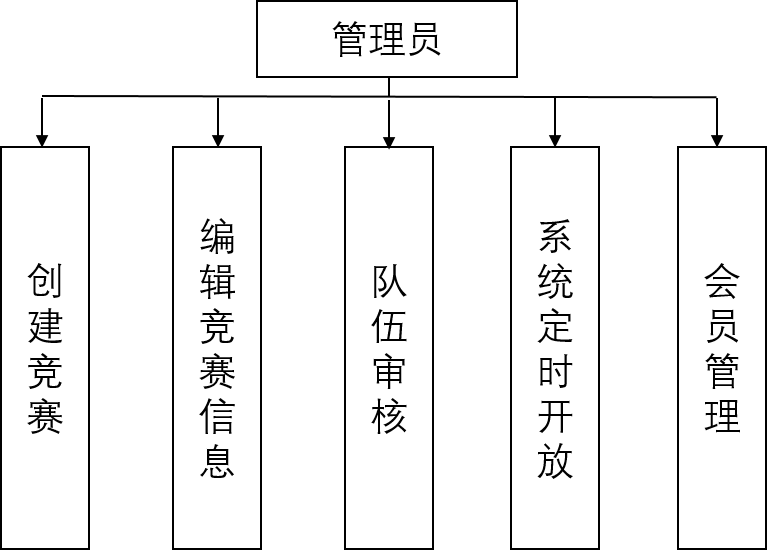
\includegraphics[width=0.7\linewidth]{images/1-1.png}
			\caption{管理员模块功能图}
		\end{figure}
		管理员模块包括在微信端的登陆、在微信端修改密码、创建比赛、会员管理、竞赛管理、开启/关闭报名权限等功能。
		
		修改密码与登陆同老师与学生。
		
		进入后会进入菜单界面,可以选择需要完成的操作。点击创建竞赛,需要填写竞赛信息,包括竞赛的名称、简介、报名时间段、比赛时间、比赛联系方式、比赛QQ群等信息。
		
		点击竞赛管理,会展示同学生端的竞赛简要信息列表,选择需要管理的竞赛,进入竞赛详情页面可以完成竞赛的管理,包括竞赛信息修改,竞赛报名开启/关闭。
		
		点击会员管理,会展示所有会员的简要信息列表,在上方可以选择展示的会员的类型,包括会员的角色、会员的部门、会员的性别、是否已审核等类型。在每条简要信息的右边有一键审核按钮。点击需要管理的会员,进入会员详细信息页面可以完成会员的管理,包括会员信息修改,审核通过或未通过。
		
		点击队伍管理,会展示所有队伍的简要信息列表。在每条简要信息的右边有一键审核按钮。点击需要管理的队伍,进入会员详细信息页面可以完成队伍的管理,包括队伍信息修改,审核通过或未通过。
		
		%%%%%%%%%%%%%%%%%%%%%%%%%%%%%%%%%%%%%%%%%%%%%%%%%%%%%%%%%%%%%%%%%%%%%%%%%%%%%%%%
		\section{详细设计与实现}
		
		\subsection{环境配置}
		\subsubsection{小程序注册}
		在微信公众平台官网首页(mp.weixin.qq.com)进入小程序注册入口,根据需求选择注册的账号类型,本文由于没有企业资质,故选择“个人”账号类型。根据流程填写邮箱和密码,并登陆邮箱激活账号,接着完成信息补充流程,将主体信息和管理员信息进行完善。其中企业、政府、媒体、其他组织类型账号需要进行微信认证后才能正常使用。此微信小程序基本信息如图4-1所示:
		
		\begin{figure}[!htb]
			\centering
			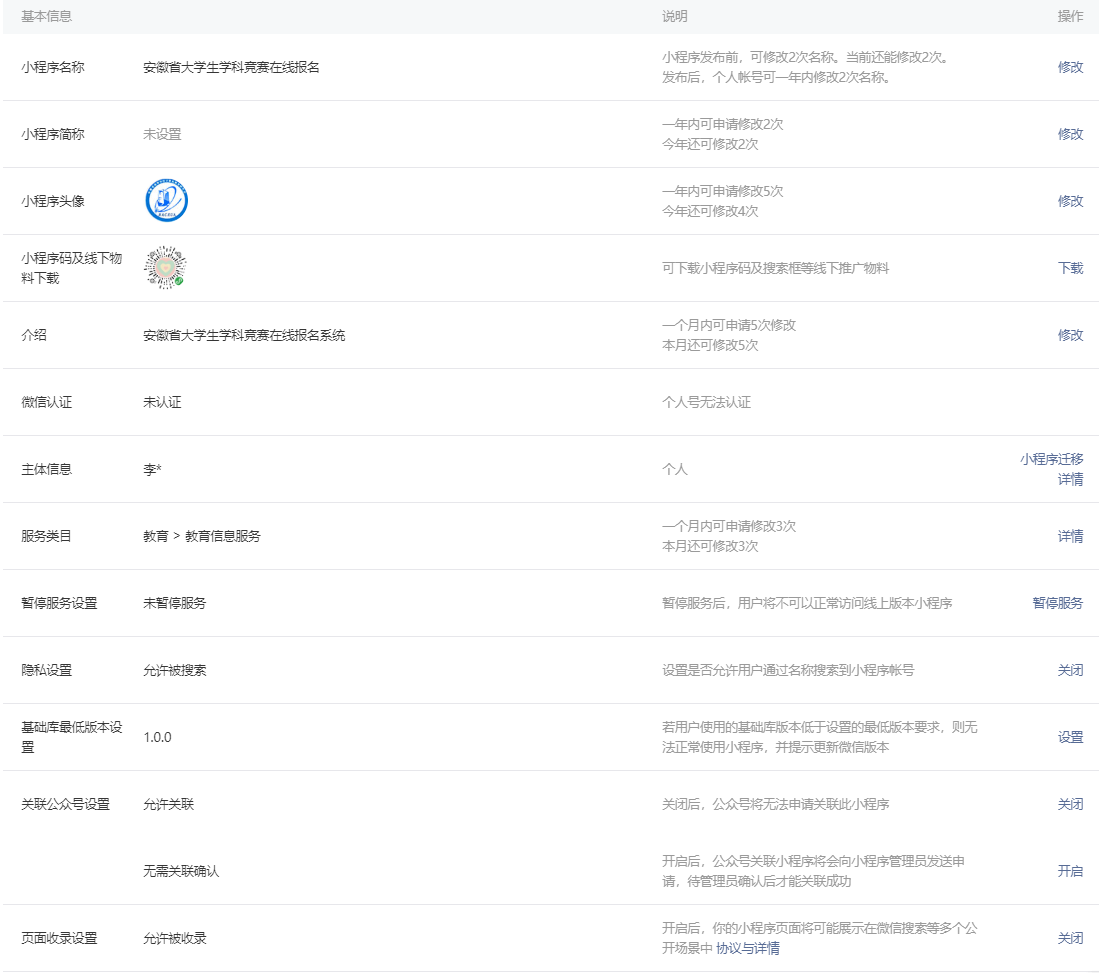
\includegraphics[width=1.0\linewidth]{images/2.jpg}
			\caption{小程序基本信息}
		\end{figure}
		
		使用者可通过扫描下方小程序码使用此移动学习平台,也可在微信中进行搜索。
		
		\begin{figure}[!htb]
			\centering
			
\includegraphics[width=0.5\linewidth]{images/3.jpg}
			\caption{小程序码}
		\end{figure}
		
		\subsubsection{开发环境与开发工具}
		微信小程序需要先在本地进行开发,开发完成后需要上传到微信官方进行审核,审核通过后才可以发布,发布后才可以被下载使用。本小程序的开发环境如下表所示:
		
		\begin{center}
			\begin{table}[!htb]
				\centering
				\caption{开发环境}
				\begin{tabular}{ccccc}
					\hline
					环境                      				&详细信息\\ \hline
					\multirow{1}{*}{PC操作系统} 				&windows10 版本号1803\\ \hline
					\multirow{1}{*}{微信web开发者工具}     	&v1.02.1803210\\ \hline
					\multirow{1}{*}{python环境}     			&python3.5.1\\ \hline
					\multirow{1}{*}{pycharm}  				&191.6605.12\\ \hline
					\multirow{1}{*}{sqlserver}    			&sqlserver12.01\\ \hline
					\multirow{1}{*}{参考文档}    			&CSS、WXML、JS、微信小程序APIv2.7.0\\ \hline
				\end{tabular}
			\end{table}
		\end{center}
		
		小程序的开发需要参考微信官方提供的微信小程序开发文档。此文档包含对于微信小程序开发的简易教程、框架介绍、组件系统、API接口、工具等项目,对于微信小程序的开发工作必不可少,开发者可以在此文档中找到所需的帮助。另外,对于WXSS(即微信样式表,WeiXinStyleSheet,)和开发过程中所需的JavaScript开发文档,需参考Mozilla Developer Network 中的JavaScript文档。
		
		\subsubsection{服务器软件硬件环境}
		(一)硬件环境
		因本系统测试成功后将部署在研究会现有的硬件环境上,在此只列出测试用服务器硬件环境。
		\begin{center}
			\begin{table}[!htb]
				\centering
				\caption{服务器硬件配置表}
				\begin{tabular}{ccccc}
					\hline
					名称                      				&详细信息\\ \hline
					\multirow{1}{*}{CPU} 					&4核\\ \hline
					\multirow{1}{*}{内存}     				&8GB\\ \hline
					\multirow{1}{*}{带宽}     				&1Mbps\\ \hline
					\multirow{1}{*}{硬盘}    				&500G\\ \hline
					\multirow{1}{*}{内网IP}  				&172.18.72.21\\ \hline
					\multirow{1}{*}{操作系统}    			&ubuntu18.04\\ \hline
				\end{tabular}
			\end{table}
		\end{center}
		
		
		(二)软件环境
		Django是采用python语言进行编写的,在其进行部署时候需要安装python语言环境,并安装Django框架。用Apache作为动态web服务器,Nginx作为静态页面的反向代理服务器,处理HMTL页面,使用MySQL作为数据库服务器。服务器软件环境配置如表4-3所示:
		
		\begin{center}
			\begin{table}[!htb]
				\centering
				\caption{服务器软件配置表}
				\begin{tabular}{ccccc}
					\hline
					名称                     				&详细信息\\ \hline
					\multirow{1}{*}{操作系统} 			    &Ubuntu18.04\\ \hline
					\multirow{1}{*}{HTTP动态页面服务}     	&Apache3.5.4\\ \hline
					\multirow{1}{*}{HTTP静态页面服务}			&Nginx1.4.12\\ \hline
					\multirow{1}{*}{数据库}    				&sqlserver2012v11.0.3128\\ \hline
					\multirow{1}{*}{语言环境}  				&Python3.5.1\\ \hline
					\multirow{1}{*}{web框架}    			    &Django2.0.1\\ \hline
				\end{tabular}
			\end{table}
		\end{center}
		
		
		微信小程序需要先进行事前设置,设置一个或多个通信域名,小程序可以和指定域名进行网络通信,包括普通的HTTPS请求、上传文件、下载文件和WebSocket通信。配置的域名只支持https和wss协议,且设置的通信域名必须已经通过ICP备案。小程序会在发起网络请求时对配置的服务器域名所使用的https证书进行校验,如果校验失败,则无法完成请求。虽然在开发阶段可以跳过域名校验,但在正式发布小程序时,若域名不支持https,则小程序的网络连接将大受影响。因此需要给前文中的CVM服务器设置域名,域名信息如图4-3所示。同时需要将此域名解析至前文CVM服务器IP地址,域名解析如图4-4所示。域名申请并解析后需要经过ICP备案才能够申请SSL证书,具体备案信息如图4-5所示。申请域名后即可申请SSL证书,在腾讯云官方网站上,可以申请有效期为42第叫章移动学习平台的环境搭迚、关饳技术与功能开发1年的SSL证书,将证书下载解压至本地,将所需文件上传至服务器,并对Apache做出相应的修改,设置正确的SSL证书地址后,24小时内HTTPS协议将生效。SSL证书信息如图4-6所示。将域名、SSL证书设置完成后,微信小程序就可以通过HTTPS协议访问服务器中的学习内容和学习资源了。
		
		\begin{figure}[!htb]
			\centering
			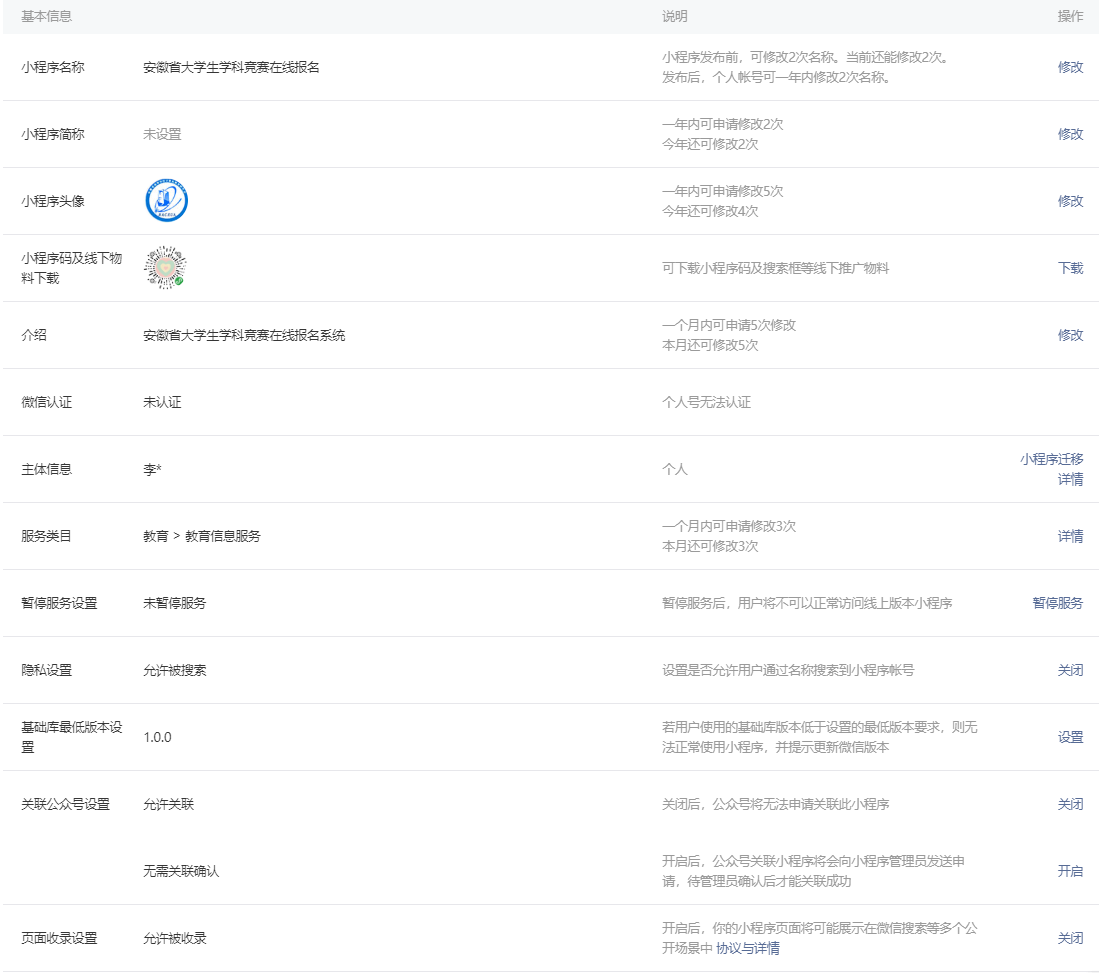
\includegraphics[width=0.5\linewidth]{images/2.jpg}
			\caption{服务器信息与证书}
		\end{figure}
		
		
		\subsection{数据库设计与实现}
		因为是在研究会现有系统上增加小程序移动办公功能,所以小程序后台直接使用研究会已有数据库,并与web端共享管理数据。微信端的设计目主要在于完成简单的移动办公操作,比如用户注册、报名、信息查询/修改、竞赛浏览等。并适合完成报名系统复杂的管理,只包含报名管理系统的一部分功能,故仅仅使用了数据库中的一部分数据表,并修改了部分数据表的项目,以适应小程序端提供的服务。使用的数据表信息列举如下。
		
		\textbf{(一)会员信息表(tblUserInfo)}
		
		为了适应小程序端的服务,在会员信息表中增加了小程userOpenID字段。登陆小程序时可以用此表端验证登陆,不用输入账号和密码。
		\begin{figure}[H]
			\centering
			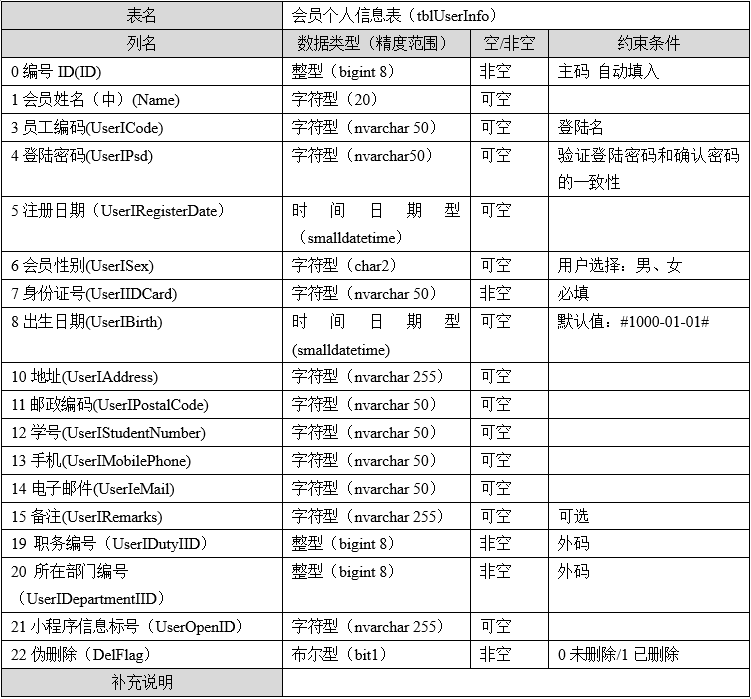
\includegraphics[width=1.0\linewidth]{images/dbtable/tblUserInfo.png}
			\caption{会员信息表}
		\end{figure}
		
		\textbf{(二)职务信息表(tblDutyInfo)}
		\begin{figure}[H]
			\centering
			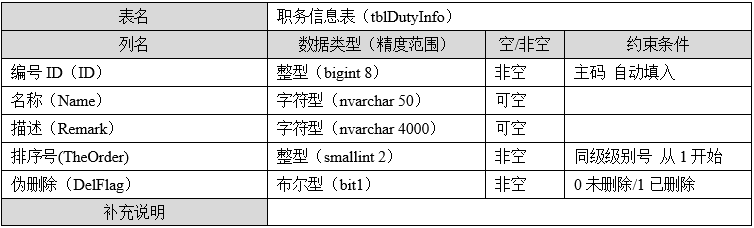
\includegraphics[width=1.0\linewidth]{images/dbtable/tblDutyInfo.png}
			\caption{职务信息表}
		\end{figure}
		
		\textbf{(三)部门信息表(tblDepartmentInfo)}
		\begin{figure}[H]
			\centering
			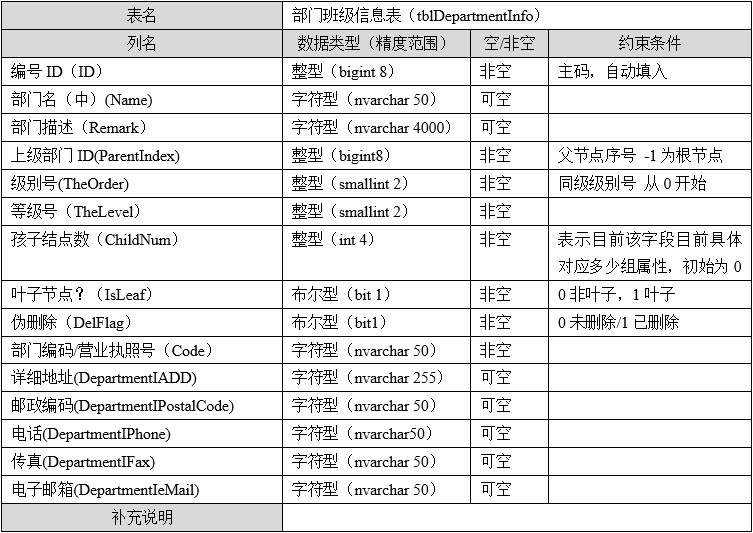
\includegraphics[width=1.0\linewidth]{images/dbtable/tblDepartmentInfo.png}
			\caption{部门信息表}
		\end{figure}
		
		\textbf{(四)竞赛信息表(tblContestInfo)}
		\begin{figure}[H]
			\centering
			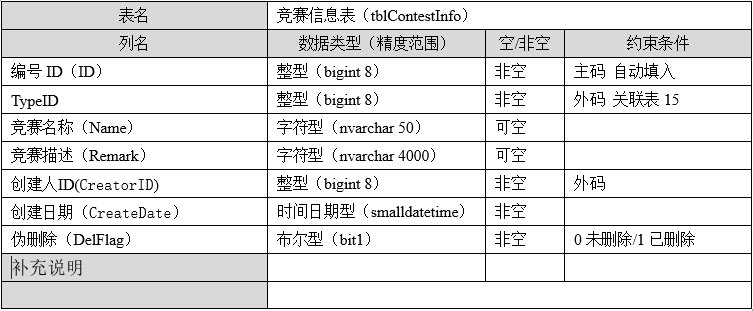
\includegraphics[width=1.0\linewidth]{images/dbtable/tblContestInfo.png}
			\caption{竞赛信息表}
		\end{figure}
		
		\textbf{(五)竞赛类型表(tblContestType)}
		\begin{figure}[H]
			\centering
			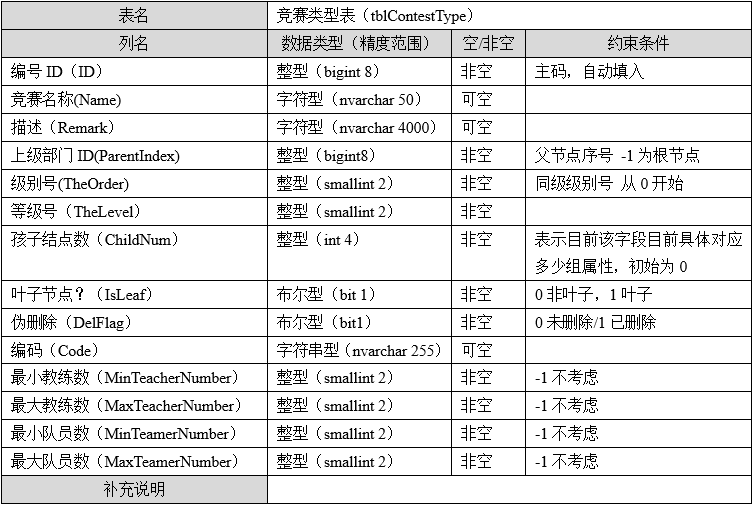
\includegraphics[width=1.0\linewidth]{images/dbtable/tblContestType.png}
			\caption{竞赛类型表}
		\end{figure}
		
		\textbf{(六)竞赛报名信息表(tblRegisterGroup)}
		\begin{figure}[H]
			\centering
			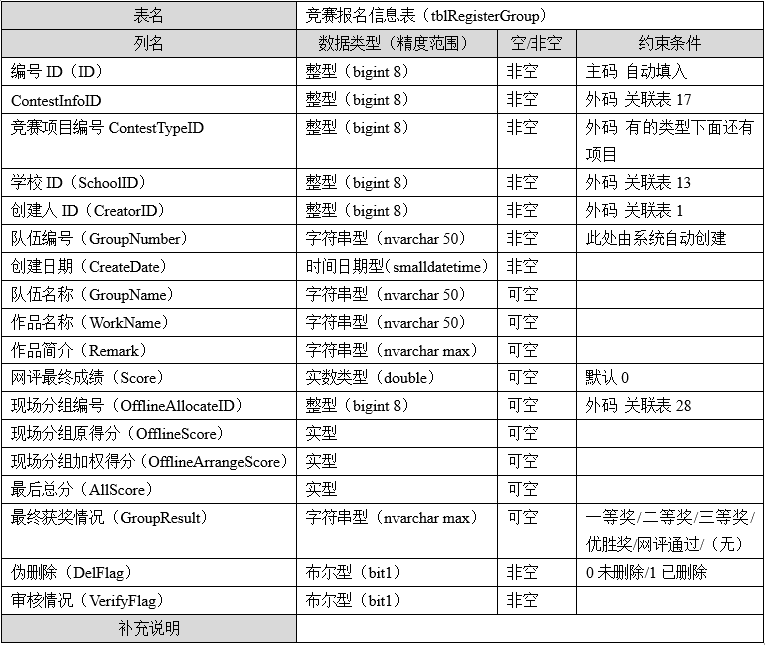
\includegraphics[width=1.0\linewidth]{images/dbtable/tblRegisterGroup.png}
			\caption{竞赛报名信息表}
		\end{figure}
		
		\textbf{(七)竞赛报名个人表(tblRegisterUser)}
		\begin{figure}[H]
			\centering
			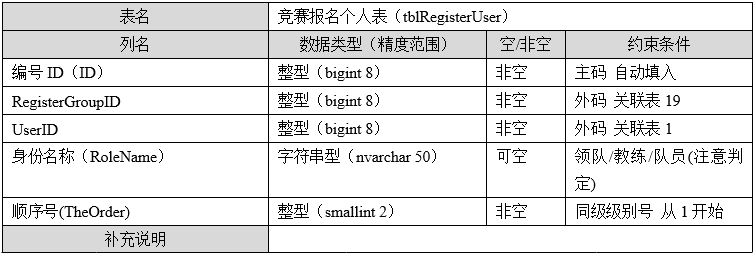
\includegraphics[width=1.0\linewidth]{images/dbtable/tblRegisterUser.png}
			\caption{竞赛报名个人表}
		\end{figure}
		
		\textbf{(八)竞赛作品信息表(tblGroupWorkInfo)}
		\begin{figure}[H]
			\centering
			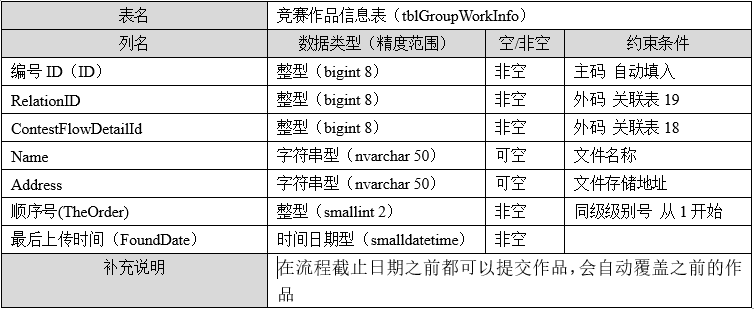
\includegraphics[width=1.0\linewidth]{images/dbtable/tblGroupWorkInfo.png}
			\caption{竞赛作品信息表}
		\end{figure}
		
		\subsection{各功能模块详细设计与实现}
		
		\subsubsection{登陆/注册模块}
		
		(一)注册页面\\
		(二)登陆页面\\
		(三)小程序页面\\
		
		\subsubsection{老师功能模块}
		
		(一)菜单栏页面\\
		(二)竞赛查看\\
		(三)竞赛队伍管理\\
		(四)创建队伍\\
		(五)报名比赛界面\\
		
		\subsubsection{学生功能模块}
		
		(一)菜单栏页面\\
		(二)浏览比赛项目\\
		(三)提交作品\\
		
		\subsubsection{管理员功能模块}
		
		(一)菜单栏界面\\
		(二)创建竞赛\\
		(三)编辑竞赛信息\\
		(四)队伍审核\\
		(五)系统定时开放\\
		(六)会员管理\\
		
		%%%%%%%%%%%%%%%%%%%%%%%%%%%%%%%%%%%%%%%%%%%%%%%%%%%%%%%%%%%%%%%%%%%%%%%%%%%%%%%%%%%%%%%%%%%%%%%%%%%%%%%%%
		
		
		\subsection{关键技术实现}
		
		\subsubsection{微信小程序接入}
		(一)填写服务器配置 
		
		在微信公众平台小程序管理页面填写详细的服务器配置,接入小程序信息如图4-7所示。其中,URL是开发者用来接收微信消息和事件的接口地址;token可以任意填写,但尽量使用一些有意义的词句,token用以生成签名(signature),服务器会对己存储的token与接口URL中包含的token进行比对,以验证安全性;而EncodingAESKey随机生成,作消息加密密钥之用。
		
		\begin{figure}[!htb]
			\centering
			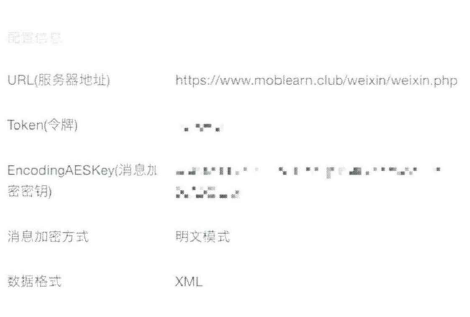
\includegraphics[width=0.5\linewidth]{images/4.jpg}
			\caption{微信小程序接入信息}
		\end{figure}
		
		(二)验证服务器地址的有效性
		
		微信验证代码端\footnote{微信验证代码端}
		\begin{minted}[
		frame=lines,
		framesep=2mm,
		baselinestretch=1.2,
		fontsize=\footnotesize,
		linenos
		]{python}
		
		def code2session(appid,code):
		API = 'https://api.weixin.qq.com/sns/jscode2session'
		params = 'appid=%s&secret=%s&js_code=%s&grant_type=authorization_code' % \
		(appid, backend.settings.WX_APP_SECRET, code)
		url = API + '?' + params
		response = requests.get(url=url,proxies=proxy.proxy())
		data = json.loads(response.text)
		return data
		\end{minted}
		
		% 微信返回数据格式\footnote{微信返回数据格式}
		% \begin{minted}[
		%     frame=lines,
		%     framesep=2mm,
		%     baselinestretch=1.2,
		%     fontsize=\footnotesize,
		%     linenos
		% ]{txt}
		% {
		%   "session_key": "JmRNs6uPEpFzlMRmg4NqJQ==",
		%   "expires_in": 7200,
		%   "openid": "oXSML0ZH05BItFTFILfgCGxXxxik"
		% }
		% \end{minted}
		
		(三)依据接口文档实现具体功能
		
		在URL有效性验证后,就可以成为小程序开发者,开发者之后就可以进行具体的设计和实现,返回使用者的请求数据,并提供各种服务。
		
		\subsubsection{Restful API接口设计}
		REST中规定了六种类型的请求方式:GET、POST、PUT、DELETE、HEAD、OPTIONS,正好与CRUD(Create-Retrieve-Update-Delete,增删改查)四种操作相对应,例如,GET(查)、POST(增)、PUT(改)、DELETE(删)。本系统的Tbluserinfo表信息的url操作基于restful请求,实现如下:
		
		\begin{center}
			\begin{table}[!htb]
				\centering
				\caption{Restful简表}
				\begin{tabular}{ccccc}
					\hline
					REST请求                    				  & 描述\\ \hline
					\multirow{1}{*}{GET:/Tbluserinfo} 		  &获取所有用户的信息\\ \hline
					\multirow{1}{*}{GET:/Tbluserinfo/001}     &获取ID为001的用户信息\\ \hline
					\multirow{1}{*}{PUT:/Tbluserinfo/001}     &更新ID为001的用户信息\\ \hline
					\multirow{1}{*}{DELETE:/Tbluserinfo/001}  &删除ID为001的用户信息\\ \hline
					\multirow{1}{*}{POST:/Tbluserinfo}        &创建新用户用户信息\\ \hline
				\end{tabular}
			\end{table}
		\end{center}
		
		
		% 获取用户信息表返回数据\footnote{获取用户信息表返回数据}
		% \begin{minted}[
		% 	frame=lines,
		% 	framesep=2mm,
		% 	baselinestretch=1.2,
		% 	fontsize=\footnotesize,
		% 	linenos
		% ]{}
		
		% {
		% 	HTTP/1.1:200,
		% 	Content-Type: application/json,
		% 	Content-Length: 234,
		% 	data:
		% 	{
		% 		"url":"/api/Tbluserinfo/1",
		% 		"method":"get",
		% 		"data":[
		% 			{
		% 				"username":"shilei"
		% 			}
		% 		]
		% 	}
		% }
		% \end{minted}
		
		%用户信息表操作使用了Django提供的基于类的视图的restfulAPI映射,基于类的通用视图被开发出来是为了解决视图中繁重的代码,它提供一个工具箱并支持多重继承,随着它的应用,它的可扩展性和灵活性远超基于函数的通用视图。基于类的通用视图是基于函数的通用视图的质的飞跃,而不仅仅是改进。
		
		%Django的URL解析器需要将request和相应的参数传递给一个可调用的函数,而不是一个类。所以class-based view提供一个类方法:view()来解决这个问题,view()方法可以把类当做函数来调用。view创建一个类实例,然后调用它的dispatch方法,dispatch分析出request是GET、POST或者其他,然后将request匹配给相应的函数,比如将POST请求匹配给post()函数,如果给函数没有定义的话,将引发HttpResponseNotAllowed错误。
		
		会员表路由配置\footnote{会员(Tbluserinfo)表路由配置}
		\begin{minted}[
		frame=lines,
		framesep=2mm,
		baselinestretch=1.2,
		fontsize=\footnotesize,
		linenos
		]{python}
		
		# urls.py
		from Django.urls import path
		from user import views
		
		urlpatterns = [
		path('getUserData', views.UserView.as_view()),
		path('updateUserData',views.UserView.as_view()),
		path('createUser',views.UserView.as_view()),
		path('isExist',views.isExist)
		]
		\end{minted}
		
		用户信息表操作代码实现\footnote{用户信息表RestfulAPI代码实现}
		\begin{minted}[
		frame=lines,
		framesep=2mm,
		baselinestretch=1.2,
		fontsize=\footnotesize,
		linenos
		]{python}
		
		# urls.py
		from Django.http import HttpResponse
		from Django.http import JsonResponse
		from Django.views import View
		from app01.models import Tbluserinfo
		
		class UserView(View, CommonResponseMixin):
		# 获取用户信息
		def get(self, request):
		ID=request.session.get('ID')
		data=Tbluserinfo.objects.filter(id=ID).values()
		message = 'get user info success'
		response = CommonResponseMixin.wrap_json_response(code=ReturnCode.SUCCESS, data=list(data))
		return JsonResponse(response, safe=False)
		
		#修改信息
		def put(self, request):
		ID = request.session.get('ID')
		received_body = request.body.decode('utf-8')
		received_body = eval(received_body)
		obj=Tbluserinfo.objects.filter(id=ID).update(**received_body)
		message = 'modify user info success.'
		response = CommonResponseMixin.wrap_json_response(code=ReturnCode.SUCCESS, message=message)
		return JsonResponse(response, safe=False)
		
		#新建用户
		def post(self,request):
		received_body = request.body.decode('utf-8')
		received_body = eval(received_body)
		received_body['delflag'] = '0'
		received_body['verifyflag'] = '1'
		Tbluserinfo.objects.create(**received_body)
		message = 'create new user success.'
		response = CommonResponseMixin.wrap_json_response(code=ReturnCode.SUCCESS, message=message)
		return JsonResponse(response, safe=False)
		
		#删除用户
		def delete(self,request):
		ID = request.session.get('ID')
		obj = Tbluserinfo.objects.filter(id=ID).update(delflag=1)
		message = 'delete user info success.'
		response = CommonResponseMixin.wrap_json_response(code=ReturnCode.SUCCESS, message=message)
		return JsonResponse(response, safe=False)
		\end{minted}
		
		\subsubsection{Django 路由分配系统}
		
		本系统的路由分配标准使用的restfulAPI设计标准,根路由配置如下表所示,用户信息表的路由配置如下下面的表所示:
		
		小程序后台路由函数\footnote{小程序后台采用Django URL路由分发模块进行路由}
		\begin{minted}[
		frame=lines,
		framesep=2mm,
		baselinestretch=1.2,
		fontsize=\footnotesize,
		linenos
		]{python}
		
		#server.urls.py
		from Django.conf.urls import url
		from Django.contrib import admin
		from Django.urls import path, include
		
		urlpatterns = [
		path('admin/', admin.site.urls),
		url(r'^app01/', include('app01.urls')),
		url(r'^login/',include('login.urls')),
		url(r'^auth/',include('authorization.urls')),
		url(r'^user/',include('user.urls')),
		url(r'^department/',include('department.urls')),
		url(r'^contest/',include('contest.urls')),
		url(r'^group/',include('group.urls')),
		]
		
		############################################
		
		#user.urls.py
		from Django.urls import path
		from user import views
		
		urlpatterns = [
		path('getUserData', views.UserView.as_view()),
		path('updateUserData',views.UserView.as_view()),
		path('createUser',views.UserView.as_view()),
		path('isExist',views.isExist)
		]
		\end{minted}
		
		\subsubsection{Django-ORM数据库操作}
		在Django中model是数据的单一、明确的信息来源。它包含了存储的数据的重要字段和行为。通常,一个模型(model)映射到一个数据库表.每个模型都是一个Python类,它是Django.db.models.Model的子类。模型的每个属性都代表一个数据库字段。综上所述,Django为您提供了一个自动生成的数据库访问API。
		
		因为本系统使用研究会网站已有的数据库文件,所以可以直接使用以下inspectdb命令进行数据库model的反向生成。生成时可以指定生成模块的位置。
		
		\textit{python manage.py inspectdb > demo/models.py}
		
		Tbluserinfo Model类\footnote{使用inspectdb命令数据库反向生成的model}
		\begin{minted}[
		frame=lines,
		framesep=2mm,
		baselinestretch=1.2,
		fontsize=\footnotesize,
		linenos
		]{python}
		
		class Tbluserinfo(models.Model):
		id = models.BigAutoField(db_column='ID', primary_key=True) 
		usericode = models.TextField(db_column='UserICode', blank=True, null=True) 
		useripsd = models.TextField(db_column='UserIPsd', blank=True, null=True) 
		useriregisterdate = models.DateTimeField(db_column='UserIRegisterDate', blank=True, null=True)  
		userisex = models.CharField(db_column='UserISex', max_length=2, blank=True, null=True)
		useriidcard = models.TextField(db_column='UserIIDCard', blank=True, null=True)  
		useribirth = models.DateTimeField(db_column='UserIBirth', blank=True, null=True)  
		useriaddress = models.TextField(db_column='UserIAddress', blank=True, null=True)  
		useripostalcode = models.TextField(db_column='UserIPostalCode', blank=True, null=True)  
		useristudentnumber = models.TextField(db_column='UserIStudentNumber', blank=True, null=True)  
		userimobilephone = models.TextField(db_column='UserIMobilePhone', blank=True, null=True)  
		useriemail = models.TextField(db_column='UserIeMail', blank=True, null=True)  
		useridutyiid = models.ForeignKey(Tbldutyinfo, models.DO_NOTHING, db_column\
		='UserIDutyIID', blank=True, null=True)  
		useridepartmentiid = models.ForeignKey(Tbldepartmentinfo, models.DO_NOTHING, db_column='UserIDepartmentIID', blank=True, null=True)  
		name = models.TextField(db_column='Name', blank=True, null=True)  
		remark = models.TextField(db_column='Remark', blank=True, null=True)  
		delflag = models.BooleanField(db_column='DelFlag')  
		verifyflag = models.BooleanField(db_column='VerifyFlag')  
		wholedepartmentname = models.TextField(db_column='WholeDepartmentName', blank=True, null=True)  
		
		class Meta:
		managed = False
		db_table = 'tblUserInfo'
		
		\end{minted}
		
		%%%%%%%%%%%%%%%%%%%%%%%%%%%%%%%%%%%%%%%%%%%%%%%%%%%%%%%%%%%%%%%%%%%%%%%%%%%%%%%%%%%%%%%%%%%%%%%
		
		%\subsection{后端日志系统实现}
		%本系统需要上线运行,需要记录系统中硬件、软件和系统问题的信息,同时还可以监视系统中发生的事件。用户可以通过它来检查错误发生的原因,或者寻找受到攻击时攻击者留下的痕迹。
		%%%%%%%%%%%%%%%%%%%%%%%%%%%%%%%%%%%%%%%%%%%%%%%%%%%%%%%%%%%%%%%%%%%%%%%%%%%%%%%%%%%%%%%%%%%%%%%
		
		\section{总结和展望}
		\subsection{总结}
		经过三个月的工作,从最初的选题到中期的设计再到最后的开发实现,毕业设计终于定稿完成,自己独自一人开发的经历对我收益匪浅,从任务开始的需求分析,不断的去登陆现有系统网站进行体验,翻看现有数据库与数据库设计资料,以及现有系统的部分源码,让我对整个系统的需求有全面的认识,对各角色的分工有了详细的了解。又因为微信小程序是自己没有接触过的全新的技术,对于开发时间与难度没有很好的估计,导致后期开发缓慢甚至停滞。并且在系统没有设计好的时候就开始了代码实现十分没有规划,导致后期重构了两次。整个过程锻炼了我独立思考的能力,对一个软件的开发流程有了更加深刻的理解,并且明白了在正式编码前对项目进行详细完备的设计是十分重要的。在整个过程中,不断完善系统的想法,一步步实现最终的报名系统。
		
		在完成本项目的过程中,我遇到很多问题,在解决问题的过程中学校到很多知识,总结出很多宝贵的经验。
		
		(一)因为本系统的前后端都是我没有接触过的技术,所以开始本系统的第一步就是学习使用小程序技术、Django框架和restfulAPI标准以及json数据串。
		
		(二)在使用Django的ORM与sqlserver联调时出现问题,一直未能解决,不能获取到sqlserver数据,因为Django原生不支持sqlserver数据库,所以资料极少,最后是使用google搜索在stackflew上才找到答案。
		
		(三)小程序获取验证信息时也进展缓慢,我是在csdn、博客园各种博客网站上寻找验证流程,但是科学的方法应该是直接认真阅读官方文档。
		
		\subsection{展望}
		
		本次毕业设计,基本需求得到满足,实现了简单易用的大部分功能,但是此报名系统还有较大的提升空间。由于时间与个人能力有限,一些可以完善的功能还未能实现。
		
		第一,界面不够美观,此次小程序界面没有找到合适的前端模板,全是从头学起,从头写起不擅长的前端。
		
		第二,各角色功能还比较少,9宫格的功能布局可以填满,实现更多丰富的功能,甚至可以将整个web端的功能都移动到小程序端来实现,实现完全的移动办公。
	
		第三,系统优化的不够全面,在一些方面可能由于个人的思考不够缜密,部分地方存在bug。
	}
	
	% 参考文献
	{
		\clearpage % 分页
		\phantomsection % 使得hyperref目录能够跳转到正确的位置
		\addcontentsline{toc}{section}{参考文献} % 添加到目录中
		\nocite{*} % 添加所有文献
		%\bibliographystyle{gbt7714-2005} % 样式
		\bibliographystyle{bib/gbt7714-2005} % 样式
		\bibliography{bib/ref.bib}    % 文献数据库
	}
	
	% 致谢
	\begin{acknowledge}
		本论文是在指导老师XXXXXXXXXXXXXXXXXXXXXXXXXXXXXXXXXXXXXXXXXXXXXXXXXXXXXXXXXXXXXXXXXXXXXXXXXXXXXXXXXXXXXXXXXXX。
		
		XXXXXXXXXXXXXXXXXXXXXXXXXXXXXXXXXXXXXXXXXXXXXXXXXXXXXXXXXXXXXXXXXXXXXX。
	\end{acknowledge}
	
	% 附录,必要时
	\begin{appendix}
		【说明:以下内容可放在附录之内:(1) 正文内过于冗长的公式推导;(2) 方便他人阅读所需的辅助性数学工具或表格;(3) 重复性数据和图表;(4) 论文使用的主要符号的意义和单位;(5) 程序说明和程序全文。可按"附录1  XXX"、"附录2  XXX"、……,分章书写。如无需附录,请删除此页。】
	\end{appendix}
	
\end{document}
